\documentclass[a4paper, 12pt]{article}
\usepackage{config}

\title{FA576 - Prova}
\author{Renan da Silva Guedes}
\date{\today}

\begin{document}
	\maketitle
	\begin{itemize}
		\item[\textbf{(1)}] As duas equações que relacionam a tensão e deformação radiais da lei de Hooke Generalizada são
		
		\begin{equation}
			\sigma_{ij}=\dfrac{E}{1+\nu}\left(\epsilon_{ij}+\dfrac{\nu}{1-2\nu}\,\delta_{ij}\,\epsilon_{kk}\right)
		\end{equation}
		
		\begin{equation}
			\epsilon_{ij}=\dfrac{1+\nu}{E}\,\sigma_{ij}-\dfrac{\nu}{E}\,\delta_{ij}\,\sigma_{kk}
		\end{equation}
		
		\item[\textbf{(2)}] Esquemas
		
		\begin{figure}[H]
			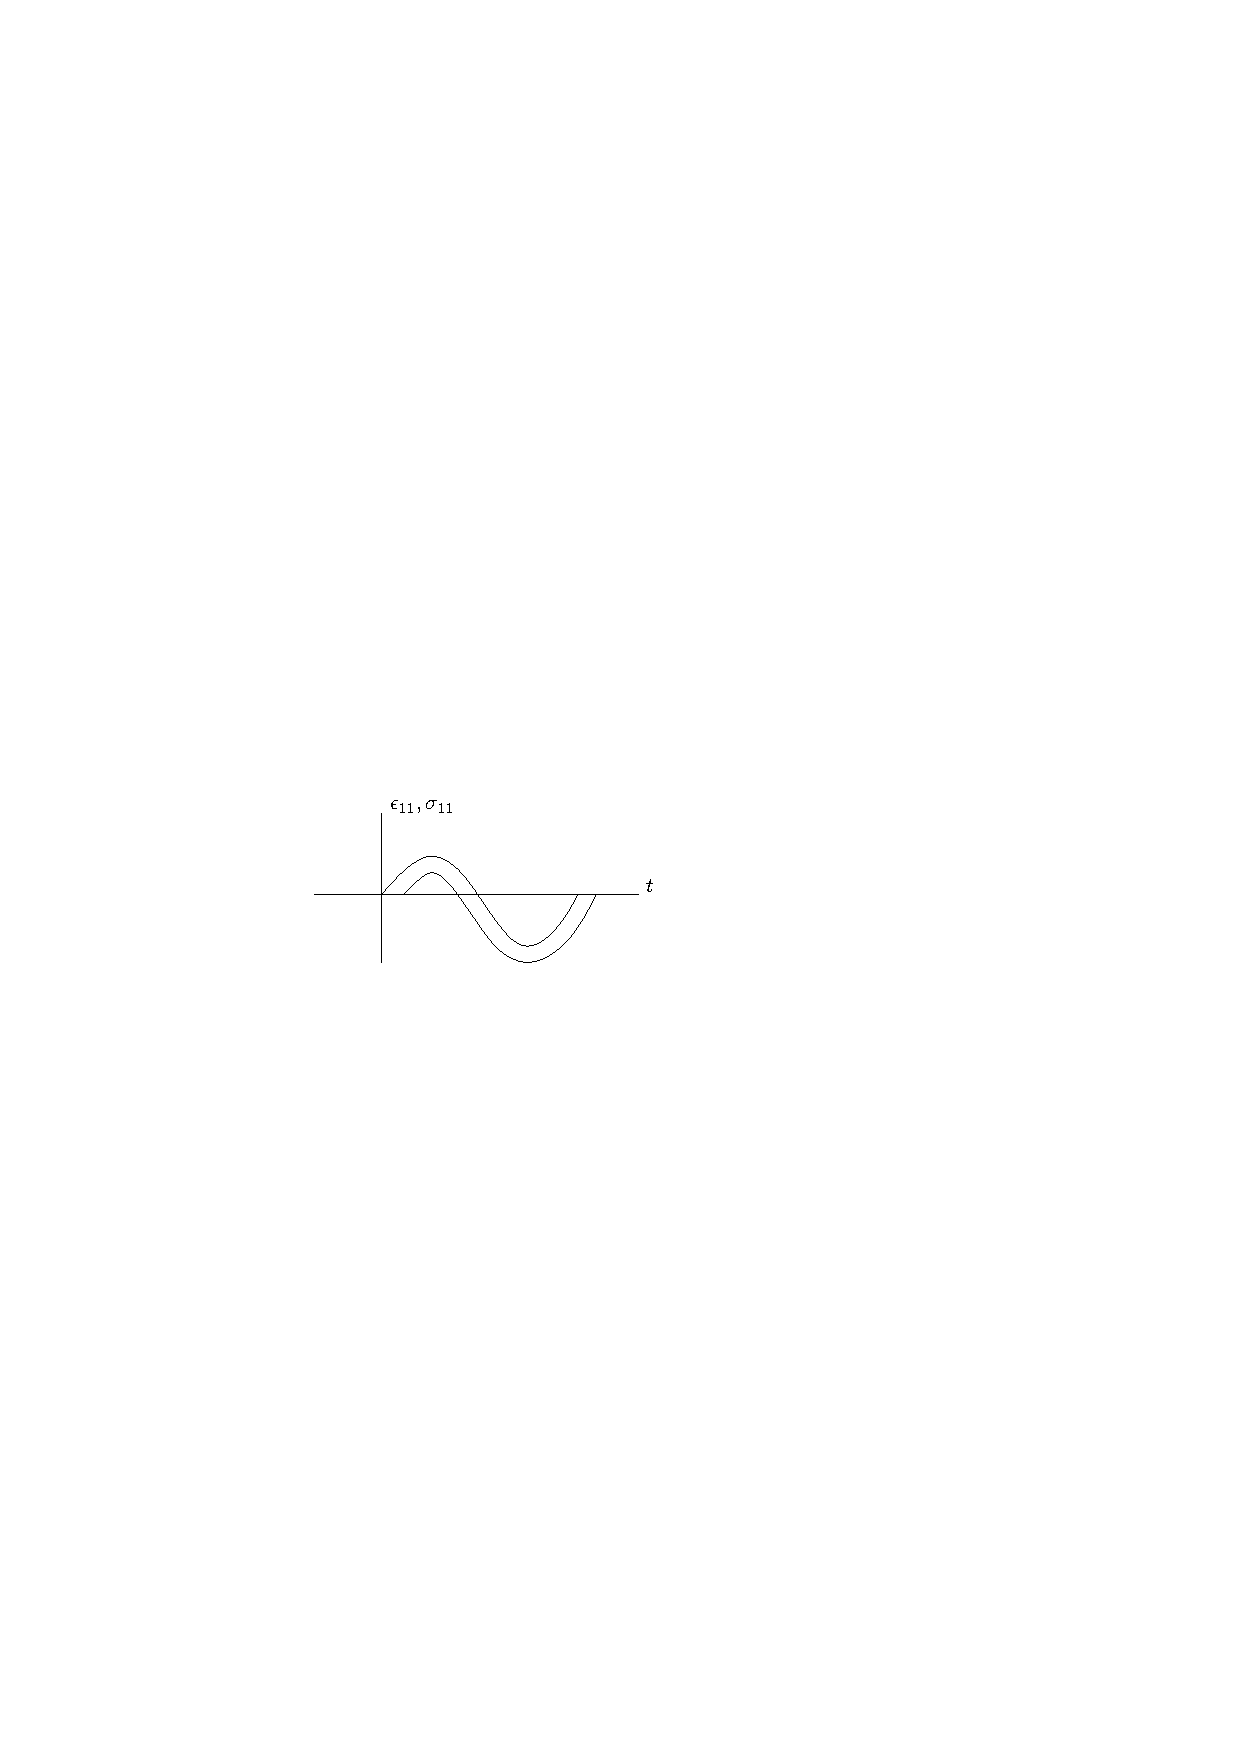
\includegraphics[scale=1.3]{images/elast}
			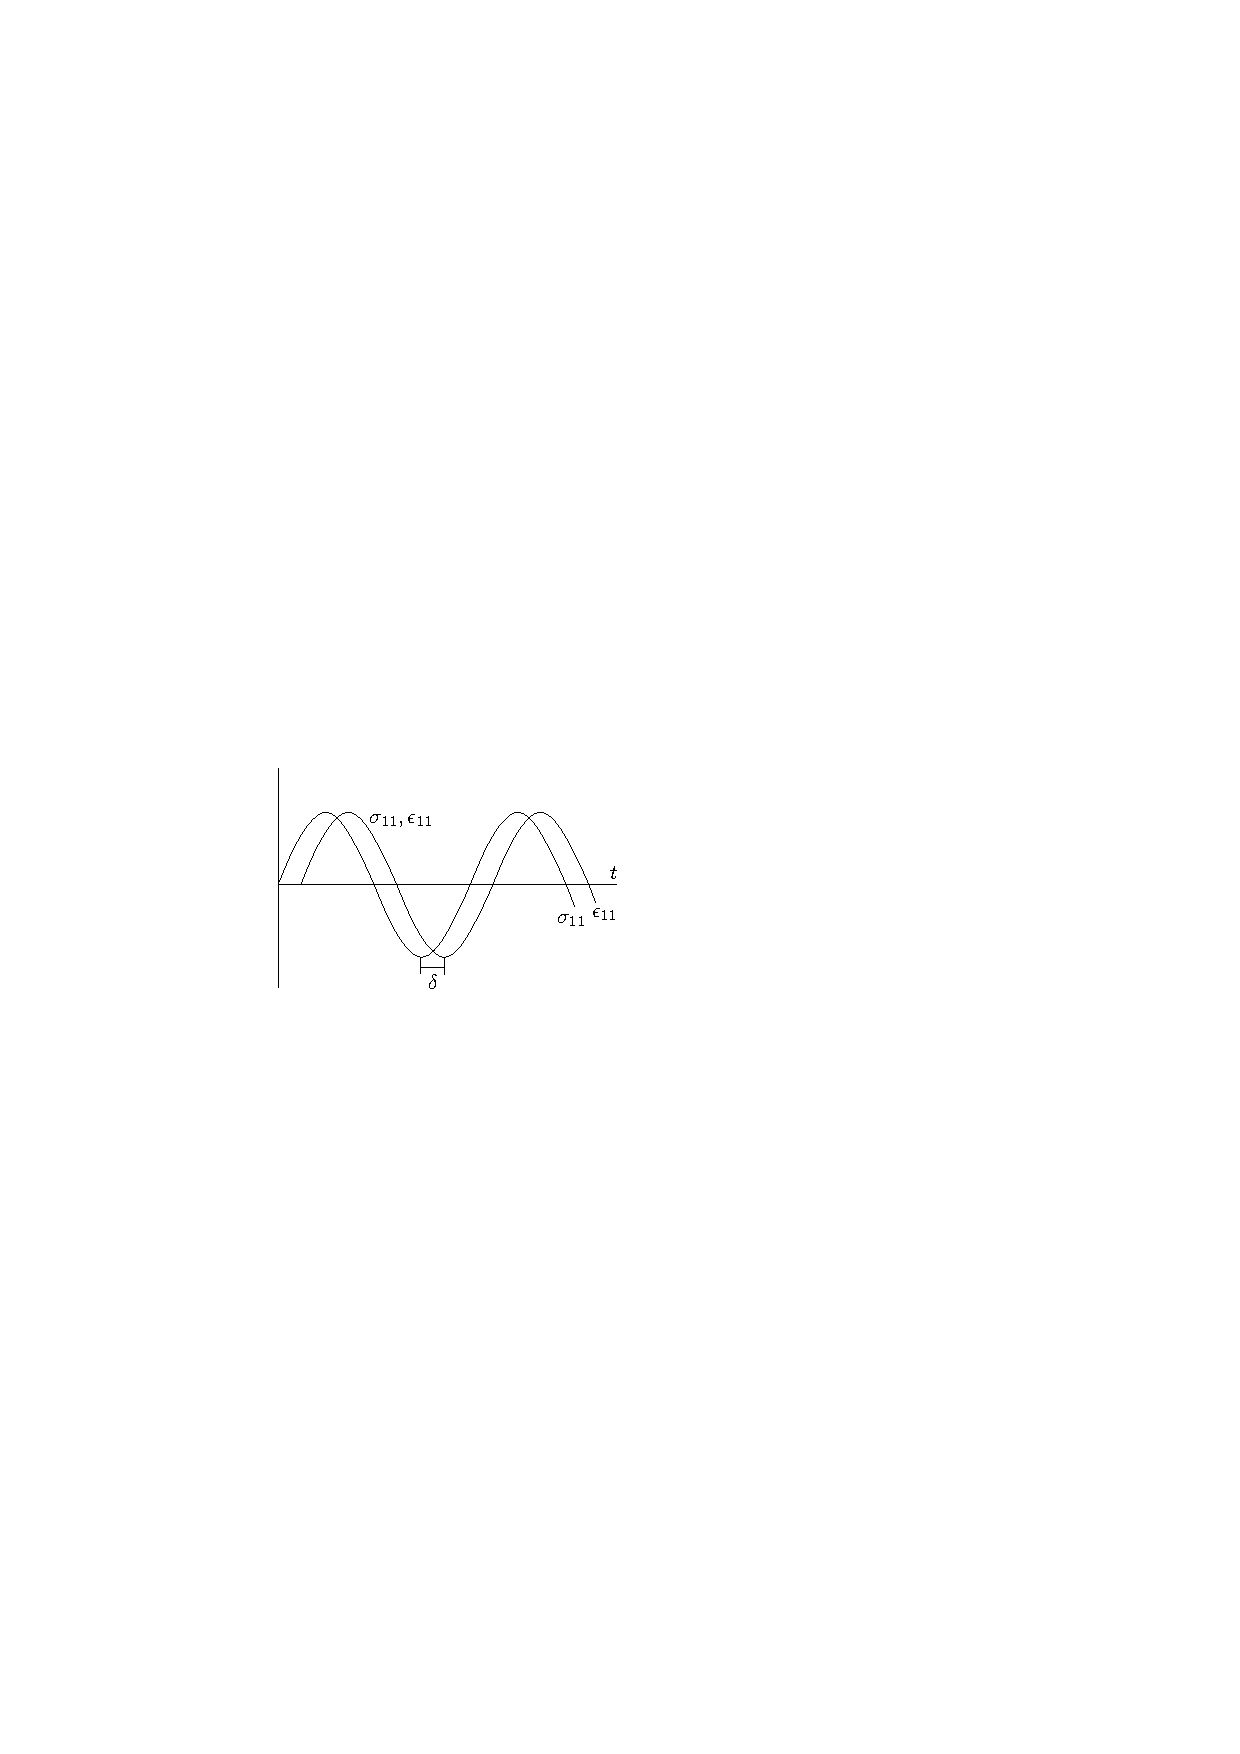
\includegraphics[scale=1.3]{images/inelast}
			\caption{Gráfico à direita ilustrando a resposta ao carregamento em um material elástico, enquanto que à esquerda, inelástico}
		\end{figure}
		
		\item[\textbf{(4)}]
		
		\begin{itemize}
			\item[\textbf{(a)}] Na equação \eqref{eq:1} abaixo, a deformação em $i$ e $j$ dadas como função de $t$ representa o \textit{strain} total. O termo $d\sigma_{ij}(t')/dt'$ representa o \textit{strees rate}, onde $\sigma_{ij}$ é o tensor $\textit{stress}$. Por fim, o termo $\psi(t-t')$ denota a função \textit{creep}.
			
			\begin{equation}
				\label{eq:1}
				\epsilon_{ij}(t)=\int\limits_{0}^{t}\dfrac{d\sigma_{ij}(t')}{dt'}\,\psi(t-t')dt'
			\end{equation}
			
			
			\item[\textbf{(b)}] Na equação \eqref{eq:2} o termo $\sigma_{ij}$ é a função \textit{stress} total dependente do tempo. O termo $d\epsilon_{ij}(t')/dt'$ é a taxa de deformação (\textit{strain rate}), onde $\epsilon_{ij}$ é o tensor \textit{strain}. A função $\phi$ é \textit{relation}.
			
			\begin{equation}
				\label{eq:2}
				\sigma_{ij}(t)=\int\limits_{0}^{t}\dfrac{d\epsilon_{ij}(t')}{dt'}\,\phi(t-t')dt'
			\end{equation}
		\end{itemize}
		
		\item[\textbf{(7)}] Para obtenção do módulo $E$ é necessário basear-se no ensaio de cargas de contato e determinação do módulo de firmeza do material. O módulo referido é o de elasticidade ou de Young. 
		
		Caso a área de contato não seja obtida é necessário lançar mão da literatura visando obter o módulo de firmeza do material estudado. Ao analisar a equação de Hertz abaixo
		
		\begin{equation}
			a=\sqrt[3]{\dfrac{3F(1-\nu^{2})\,R}{4E}}
		\end{equation}
		ao rearranjar os termos, temos que
		
		\begin{equation}
			\label{eq:hertz}
			\left(\dfrac{E}{1-\nu^{2}}\right)=\dfrac{3FR}{4a^{3}}
		\end{equation}
		dessa forma, por não possuirmos as características associadas à área de contato seria necessário aplicar somente o lado direito de \eqref{eq:hertz} visando obter o módulo $E$. Porém a consideração a ser feita seria
		
		\begin{equation}
			\textit{firmness}=\dfrac{E}{1-\nu^{2}}
		\end{equation}
		onde \textit{firmness} e $\nu$ são conhecidos.
	
		\item[\textbf{(8)}]		
		
		\begin{itemize}
			\item[\textbf{(a)}] A linearidade ou não linearidade geométrica estão vinculadas às características físicas do material ao ser submetido a esforços e solicitações. Sendo que estes podem originar deformações do material e a consequente alteração da sua estabilidade.
			\item[\textbf{(b)}] A linearidade material está vinculada às características dependentes do tempo, oriundas das mudanças físicas no interior do corpo afetando a sua uniformidade e semelhanças estruturais em toda sua porção, podendo ocasionar variação das propriedades mecânicas.
		\end{itemize}
	
		\item[\textbf{(10)}] As três equações apresentadas acima referem-se ao ensaio de compressão diametral de um corpo de prova cilíndrico. $E$ e $\nu$ representam o módulo de Young e coeficiente de Poisson, respectivamente. $Z$ é uma grandeza adimensional dada pela razão entre o raio do cilindro ($R$) e a metade da largura da área de contato. $F$ é a força máxima aplicada na deformação do corpo de prova, enquanto $D$ e $d$ são a deformação e o diâmetro do cilindro, respectivamente.
		
		\item[\textbf{(12)}] As perdas podem ser diminuídas a partir do estudo mais aprofundado envolvendo a interação das operações mecanizadas e os esforços suportados por cada material. Ou seja, deve-se haver mais especificidade e adequação entre o que o produto requer para que não sofra danos ou injúrias mecânicas e os elementos ao longo da cadeia de produção, englobando todas as variáveis pertinentes até a fase de comercializar a mercadoria.
	\end{itemize} 
\end{document}